\documentclass{article}
\usepackage[utf8]{inputenc}
\usepackage{tikz}
\usepackage{pdfpages}
\usepgflibrary{fpu}
\usepackage{ifthen}
\setlength{\parindent}{0pt}


\newcommand{\pasc}[2]{
	\pgfkeys{/pgf/fpu}
	\pgfmathparse{round(#1!/((#1-#2)!*#2!))}
	\pgfmathfloattoint{\pgfmathresult}
	\pgfmathresult
}

\begin{figure}[h]
	\centering
	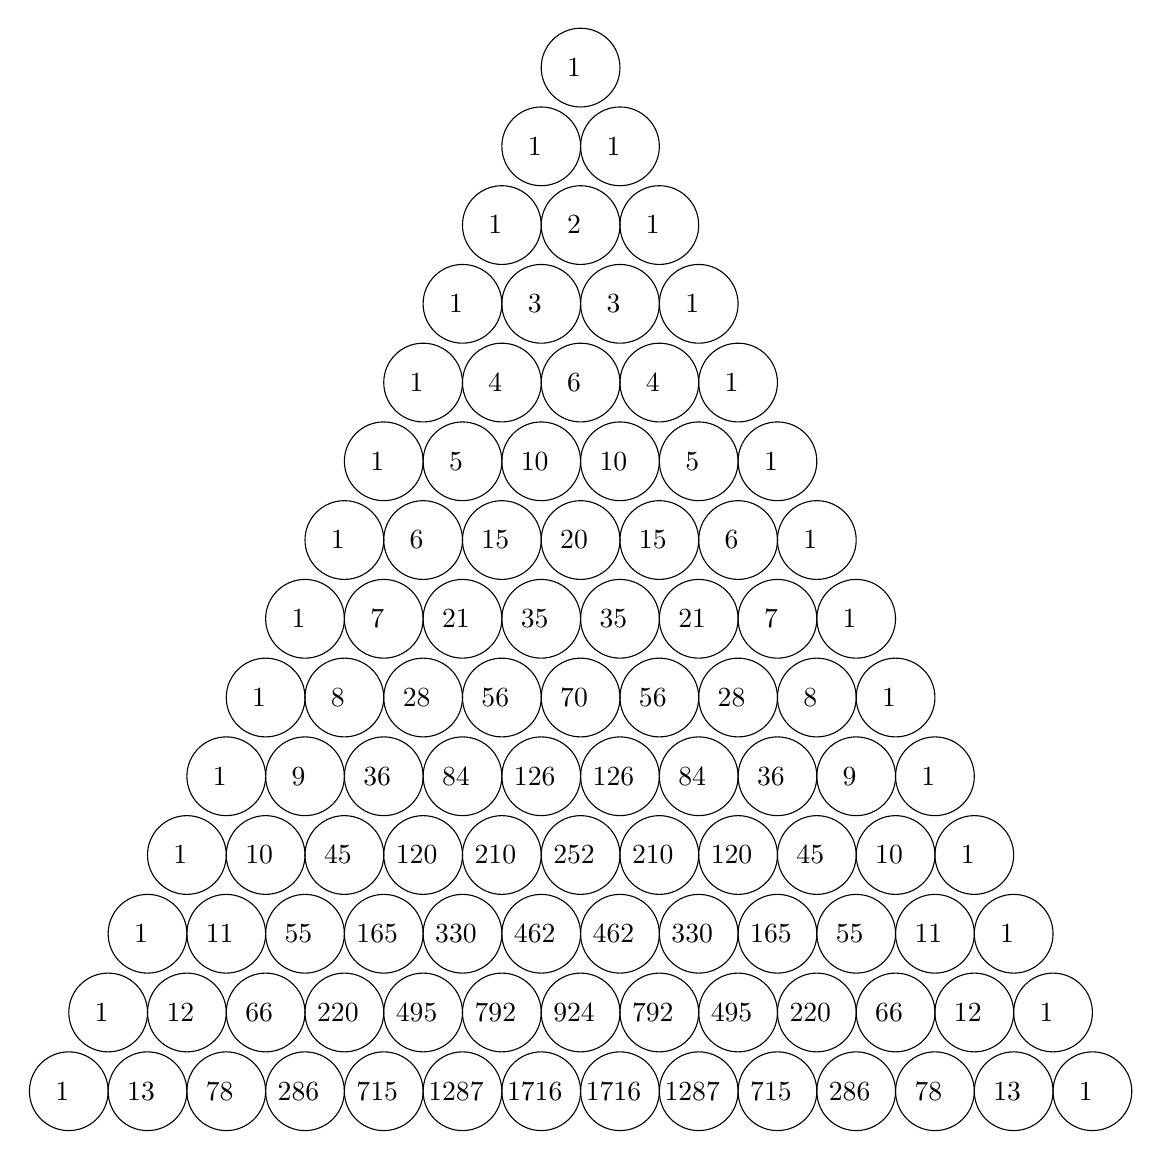
\begin{tikzpicture}
	\pgfmathsetmacro{\N}{13};
	\foreach \i in {0,...,\N}{
		\foreach \j in {0,...,\i}{
			%\pgfmathtruncatemacro{\var}{\pasc{\i}{\j}}
			\node at ({-0.5*\i+\j-0.2},-\i){\pasc{\i}{\j}};
			
			%\ifthenelse{\pasc{\i}{\j}=}{then clause}{else clause}
			% \draw ({-0.5*\i+\j-0.5},-\i+0.5) rectangle
			% ({-0.5*\i+\j-0.5},-\i-0.5);
			\draw ({-0.5*\i+\j},-\i) circle (0.5);
		}
	}
	\end{tikzpicture}
\end{figure}

